\section{moeo\-Roulette\-Select$<$ MOEOT $>$ Class Template Reference}
\label{classmoeoRouletteSelect}\index{moeoRouletteSelect@{moeoRouletteSelect}}
Selection strategy that selects ONE individual by using roulette wheel process.  


{\tt \#include $<$moeo\-Roulette\-Select.h$>$}

Inheritance diagram for moeo\-Roulette\-Select$<$ MOEOT $>$::\begin{figure}[H]
\begin{center}
\leavevmode
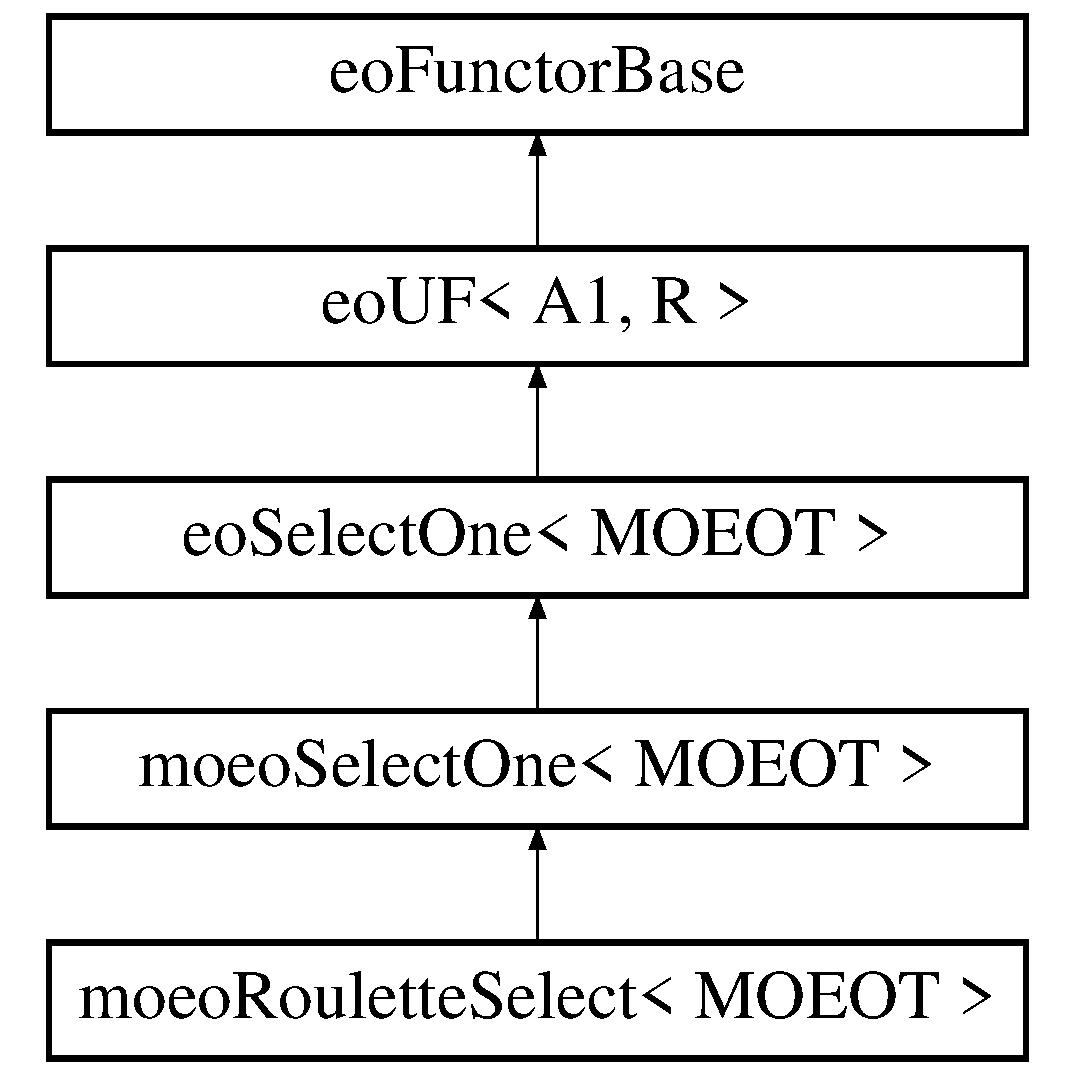
\includegraphics[height=5cm]{classmoeoRouletteSelect}
\end{center}
\end{figure}
\subsection*{Public Member Functions}
\begin{CompactItemize}
\item 
\bf{moeo\-Roulette\-Select} (unsigned int \_\-t\-Size=2)
\begin{CompactList}\small\item\em Ctor. \item\end{CompactList}\item 
const MOEOT \& \bf{operator()} (const \bf{eo\-Pop}$<$ MOEOT $>$ \&\_\-pop)
\begin{CompactList}\small\item\em Apply the tournament to the given population. \item\end{CompactList}\end{CompactItemize}
\subsection*{Protected Attributes}
\begin{CompactItemize}
\item 
double \& \bf{t\-Size}\label{classmoeoRouletteSelect_19af84fe966381cbfbe032f69ee0b42b}

\begin{CompactList}\small\item\em size \item\end{CompactList}\end{CompactItemize}


\subsection{Detailed Description}
\subsubsection*{template$<$class MOEOT$>$ class moeo\-Roulette\-Select$<$ MOEOT $>$}

Selection strategy that selects ONE individual by using roulette wheel process. 

\begin{Desc}
\item[Warning:]This selection only uses fitness values (and not diversity values). \end{Desc}




Definition at line 49 of file moeo\-Roulette\-Select.h.

\subsection{Constructor \& Destructor Documentation}
\index{moeoRouletteSelect@{moeo\-Roulette\-Select}!moeoRouletteSelect@{moeoRouletteSelect}}
\index{moeoRouletteSelect@{moeoRouletteSelect}!moeoRouletteSelect@{moeo\-Roulette\-Select}}
\subsubsection{\setlength{\rightskip}{0pt plus 5cm}template$<$class MOEOT$>$ \bf{moeo\-Roulette\-Select}$<$ MOEOT $>$::\bf{moeo\-Roulette\-Select} (unsigned int {\em \_\-t\-Size} = {\tt 2})\hspace{0.3cm}{\tt  [inline]}}\label{classmoeoRouletteSelect_4caa45f4c9d1ad2949cc14d2c21b77ea}


Ctor. 

\begin{Desc}
\item[Parameters:]
\begin{description}
\item[{\em \_\-t\-Size}]the number of individuals in the tournament (default: 2) \end{description}
\end{Desc}


Definition at line 57 of file moeo\-Roulette\-Select.h.

References moeo\-Roulette\-Select$<$ MOEOT $>$::t\-Size.

\subsection{Member Function Documentation}
\index{moeoRouletteSelect@{moeo\-Roulette\-Select}!operator()@{operator()}}
\index{operator()@{operator()}!moeoRouletteSelect@{moeo\-Roulette\-Select}}
\subsubsection{\setlength{\rightskip}{0pt plus 5cm}template$<$class MOEOT$>$ const MOEOT\& \bf{moeo\-Roulette\-Select}$<$ MOEOT $>$::operator() (const \bf{eo\-Pop}$<$ MOEOT $>$ \& {\em \_\-pop})\hspace{0.3cm}{\tt  [inline]}}\label{classmoeoRouletteSelect_573fe156daf6fdfbae96d2b54a9fc260}


Apply the tournament to the given population. 

\begin{Desc}
\item[Parameters:]
\begin{description}
\item[{\em \_\-pop}]the population \end{description}
\end{Desc}


Definition at line 73 of file moeo\-Roulette\-Select.h.

References moeo\-Roulette\-Select$<$ MOEOT $>$::t\-Size.

The documentation for this class was generated from the following file:\begin{CompactItemize}
\item 
moeo\-Roulette\-Select.h\end{CompactItemize}
